\item In the arrangement shown in Fig. 1.18 the mass of ball 1 is \(\eta = 1.8\) times as great as that of rod 2. The length of the latter is \(l = 100\) cm. The masses of the pulleys and the threads, as well as the friction, are negligible. The ball is set on the same level as the lower end of the rod and then released. How soon will the ball be opposite the upper end of the rod?
    \begin{center}
        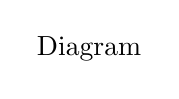
\begin{tikzpicture}
            \node at (0, 0) {Diagram};
        \end{tikzpicture}
    \end{center}